\subsubsection{Choice of technology}

As is common in web development we have used Hypertext Markup Language (HTML) to mark up the structure of the client, Cascading Stylesheets (CSS) to handle the styling/displaying of the website and JavaScript for the behavior of the website (event listeners etc.). We have supplemented our JavaScript with the JQuery framework, which provides facilities for DOM manipulation and cross-browser compability of event listeners. We have supplemented this with JQuery plugins for cookie handling etc.

With our client we wanted to show that our web service allows for a simple \emph{server-free} client solution and as such we have chosen to avoid server side coding completely in the client solution although our group has extensive experience in server side scripting (PHP).
This choice allows us to avoid a degree of indirection in our product, since every request goes directly from our JavaScript to the webservice instead of going to a server-side script first. We believe that cutting out the "middle man" has a positive effect on the performance of our solution.

We communicate with the webservice through a technology called Asynchronous JavaScript and XML (AJAX), which enables us to retrieve JSON data from the web service asynchronously.
Besides fetching the web service data through AJAX, we also use the technology whenever the user wants to navigate to another page in the client. This approach enables us to fetch the main part of the page asynchronously, while never actually reloading the page. This makes for a more fluid user experience, since the navigation bar and javascript variables only need to be set up once.

We have created our own framework in JavaScript, which provides the functions for navigation and the initialization of our global javascript variables. An example use of the framework is shown in Figure ~\ref{fig:ajax}.

\begin{figure}[hbt]
	\centering
	\centerline{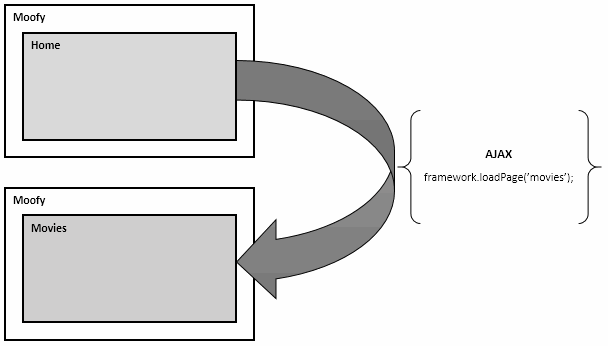
\includegraphics[scale=1]{./p1design/ajax.png}}
	\caption{Example of asynchronous page navigation through our framework.}
	\label{fig:ajax}
\end{figure}

The styled visual appearance of our client can largely be attributed to the use of the front-end framework Twitter Bootstrap, which provides the CSS styling of our navigationbars, forms, icons, buttons, etc. We chose this framework, since it allowed us to skip about a lot of manual css styling, which enables faster prototyping. As a supplement to Twitter Bootstrap we have created a JavaScript framework for outputting CSS-styled information to the user, either through success messages, error messages, or variations of modal dialog windows. This framework is used to speed up our own production speed as well as provide a consitent look and feel across the client.
A last note regarding the visual appearance of the client is the use of Gravatar (acronym for \textbf{G}lobally \textbf{R}ecognized \textbf{Avatar}), which allows Gravatar users to have their profile picture shown in our client based on their email adress.

